\clearpage
\chapter{Test}
Abschließend soll die Software getestet werden. Dazu werden Testdaten bereitgestellt. Jeder Testfall enthält den jeweiligen Vorgang, der durchzuführen ist, das zu erwartende Ergebnis bei korrektem Verhalten der Software und mögliche andere Ergebnisse bzw. Fehlverhalten, die eintreten können.

\section{Testfall 1 - Spielmodus: Gegen Computer}
\begin{figure}[!h]
	\centering
    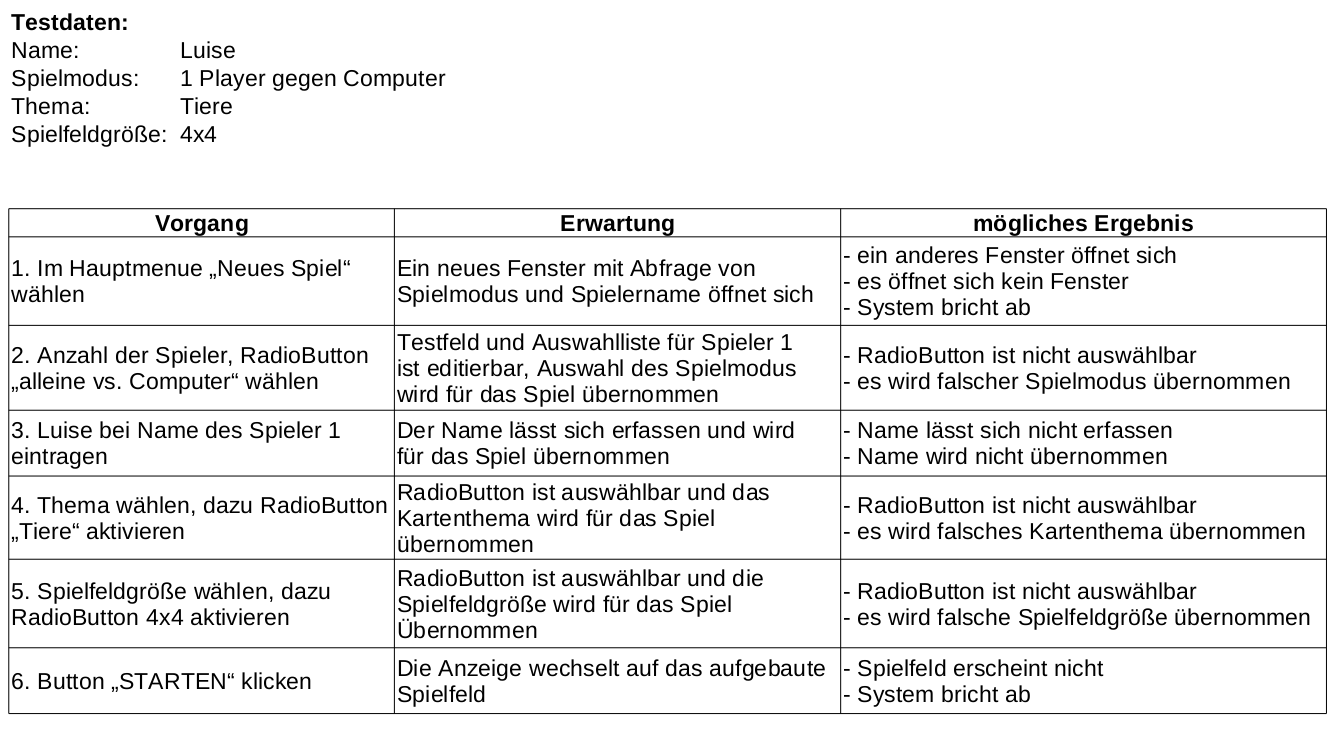
\includegraphics[width=15cm]{./Testfall1.png}
	\label{layout_gesamt}
\end{figure}

\clearpage
\section{Testfall 2 - Spielmodus: 2 Spieler}
\begin{figure}[!h]
	\centering
    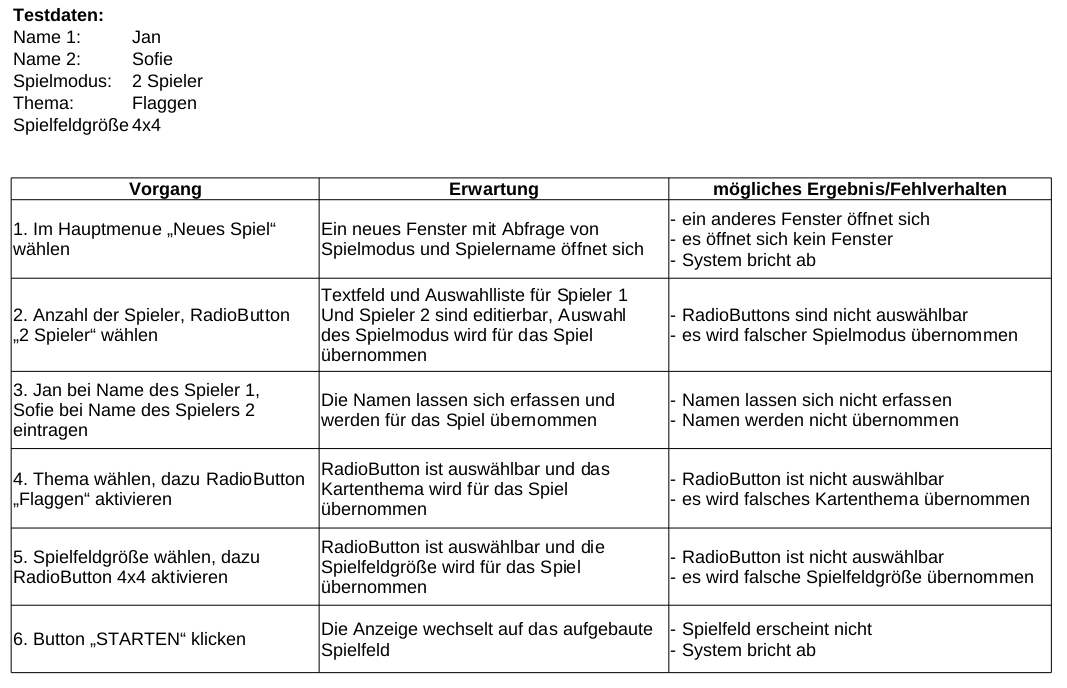
\includegraphics[width=15cm]{./Testfall2.png}
	\label{layout_gesamt}
\end{figure}

\clearpage
\section{Testfall 3 - Spieler aus Liste wählen}
\begin{figure}[!h]
	\centering
    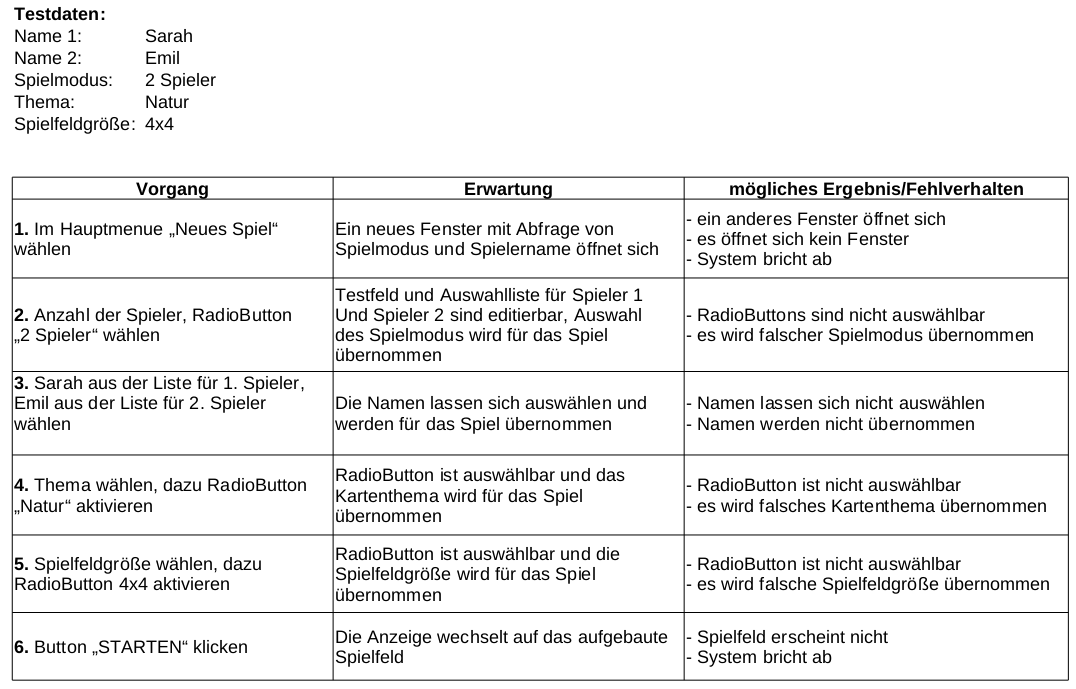
\includegraphics[width=15cm]{./Testfall3.png}
	\label{layout_gesamt}
\end{figure}

\clearpage
\section{Testfall 4 - Spielablauf testen}
\begin{figure}[!h]
	\centering
    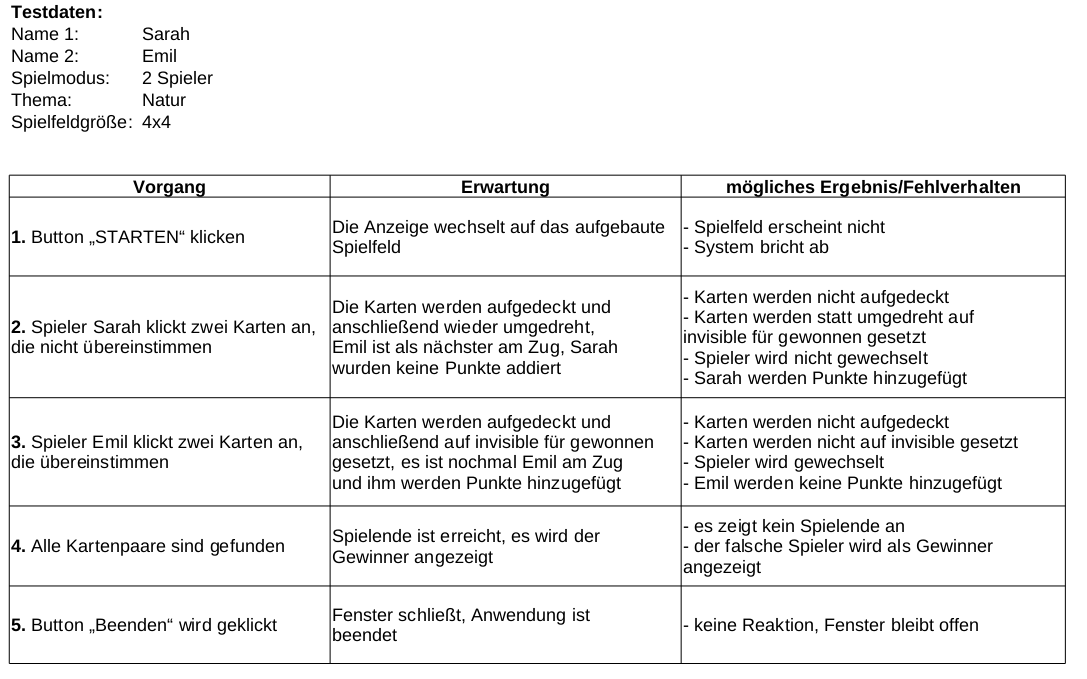
\includegraphics[width=15cm]{./Testfall4.png}
	\label{layout_gesamt}
\end{figure}

\clearpage
\section{Testfall 5 - Highscore anzeigen}
\begin{figure}[!h]
	\centering
    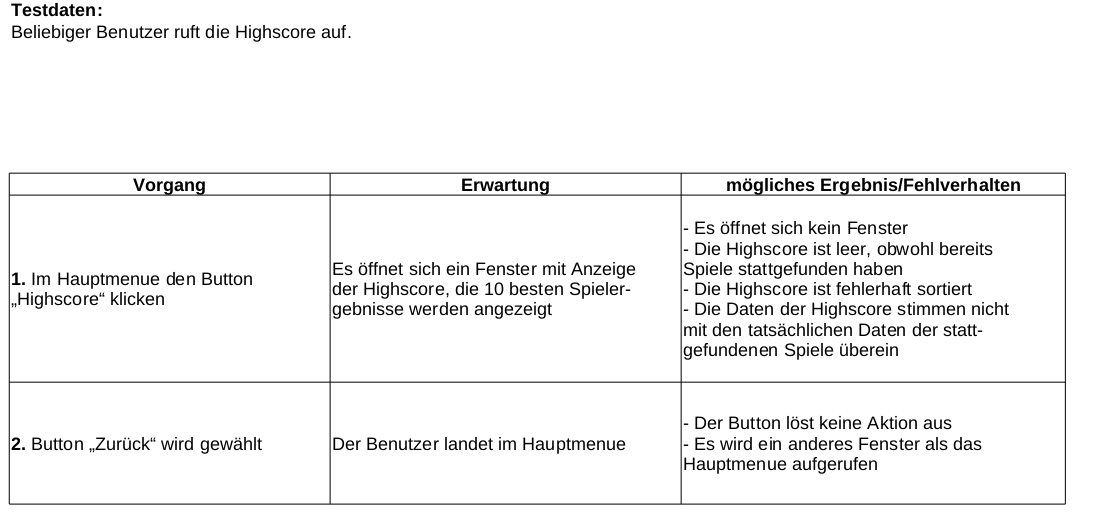
\includegraphics[width=15cm]{./Testfall5.png}
	\label{layout_gesamt}
\end{figure}
